\documentclass[english]{SPFShortReport}
\usepackage{subfigure}
\usepackage{spfFigures}
\usepackage{longtable}
\usepackage{url}
\usepackage{gensymb}
\usepackage[yyyymmdd,hhmmss]{datetime}
\reportName{Python calculation for heat pump AWHP-LEXETA}
\reportSubName{Parametric Heat Pump calculation} 
\reportDate{\today \hspace{0.1cm} at: \currenttime \hspace{0.1cm} h} 
\author{Dani Carbonell}
\address{dani.carbonell@solarenergy.ch}
\begin{document}
\begin{table}[!ht]
\begin{small}
\caption{Fitted coefficients for the heat pump.}
\begin{center}
\resizebox{12cm}{!} 
{
\begin{tabular}{l | c c } 
\hline
\hline
Coefficient &Description & \\ 
 & &$[kW]$\\ 
\hline
$PQ_{1}$ & \emph{$1^{st}$ condenser polynomial coefficient}  & 1.4130e+01    \\ 
$PQ_{2}$ & \emph{$2^{st}$ condenser polynomial coefficient}  & 5.6250e+01    \\ 
$PQ_{3}$ & \emph{$3^{st}$ condenser polynomial coefficient}  & -3.5630e+01    \\ 
$PQ_{4}$ & \emph{$4^{st}$ condenser polynomial coefficient}  & 2.9500e+02    \\ 
$PQ_{5}$ & \emph{$5^{st}$ condenser polynomial coefficient}  & -4.2000e+02    \\ 
$PQ_{6}$ & \emph{$6^{st}$ condenser polynomial coefficient}  & 0.0000e+00    \\ 
\hline
$PCOP_{1}$ & \emph{$1^{st}$ COP polynomial coefficient}  & 7.4000e+00    \\ 
$PCOP_{2}$ & \emph{$2^{st}$ COP polynomial coefficient}  & 3.7250e+01    \\ 
$PCOP_{3}$ & \emph{$3^{st}$ COP polynomial coefficient}  & -2.9000e+01    \\ 
$PCOP_{4}$ & \emph{$4^{st}$ COP polynomial coefficient}  & -3.7500e+01    \\ 
$PCOP_{5}$ & \emph{$5^{st}$ COP polynomial coefficient}  & -9.2500e+01    \\ 
$PCOP_{6}$ & \emph{$6^{st}$ COP polynomial coefficient}  & 0.0000e+00    \\ 
\hline
$\dot m_{cond}$ & 1800.00 $[kg/h]$\\ 
$\dot m_{evap}$ & 2000.00 $[kg/h]$\\ 
\hline
$COP_{nom}$ (B0W35)& 3.35 \\ 
$Q_{c,nom}$ (B0W35)& 8.26 kW\\ 
$COP_{nom}$ (B2W35)& 3.57 \\ 
$Q_{c,nom}$ (B2W35)& 8.87 kW\\ 
$COP_{nom}$ (B10W35)& 4.38 \\ 
$Q_{c,nom}$ (B10W35)& 11.05 kW\\ 
\hline
\hline
\end{tabular}
}
\label{CoefTable}
\end{center}
\end{small}
\end{table}
\begin{table}[!ht]
\begin{small}
\caption{Predicting results of the heat pump.}
\begin{center}
\resizebox{12cm}{!} 
{
\begin{tabular}{l | c c c c c c c c c c c } 
\hline
\hline
$T_{evap,in}$ &$T_{evap,out}$ &$T_{cond,in}$ &$T_{cond,out}$ &$COP$ &$Q_{cond}$ &$Q_{evap}$ &$W_{comp}$ &$\dot m_{cond}$ &$\dot m_{evap}$ &$\Delta T_{evap}$ &$\Delta T_{cond}$ \\ 
$^oC$ &$^oC$ &$^oC$ &$^oC$ &$[-]$ &$[kW]$ &$[kW]$ &$[kW]$ &kg/h &kg/h &K &K\\ 
\hline
-7.00 & -8.38 & 47.93 & 50.00 & 1.27 & 4.34 & 0.92 & 3.42 & 1800 & 2000 & 1.4 & 2.1\\ 
-7.00 & -4.69 & 55.57 & 57.50 & 0.72 & 4.05 & -1.54 & 5.59 & 1800 & 2000 & -2.3 & 1.9\\ 
-7.00 & -11.28 & 64.53 & 65.00 & -0.53 & 0.99 & 2.86 & -1.87 & 1800 & 2000 & 4.3 & 0.5\\ 
7.00 & -1.31 & 45.72 & 50.00 & 2.63 & 8.97 & 5.56 & 3.41 & 1800 & 2000 & 8.3 & 4.3\\ 
7.00 & 0.92 & 53.45 & 57.50 & 1.92 & 8.49 & 4.07 & 4.42 & 1800 & 2000 & 6.1 & 4.1\\ 
7.00 & 4.39 & 61.03 & 65.00 & 1.27 & 8.32 & 1.75 & 6.57 & 1800 & 2000 & 2.6 & 4.0\\ 
\hline
\hline
\end{tabular}
}
\label{ResultsTable}
\end{center}
\end{small}
\end{table}
\begin{figure}[!ht]
\begin{center}
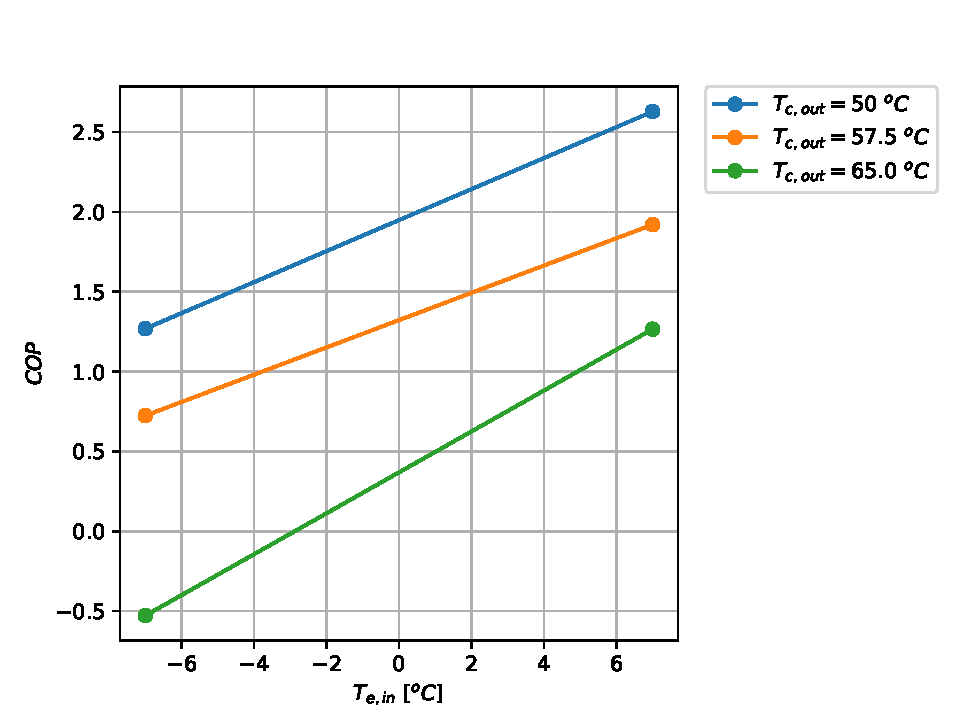
\includegraphics[width=1\textwidth]{C:/Daten/OngoingProject/TRNSYS-Polysun/HeatPumpFit/AirToWater/LEXETA/AWHP-LEXETA/AWHP-LEXETA-Cop.pdf}
\caption{COP Results for the heat pump at the selected points}
\label{COPFig}
\end{center}
\end{figure}
\begin{figure}[!ht]
\begin{center}
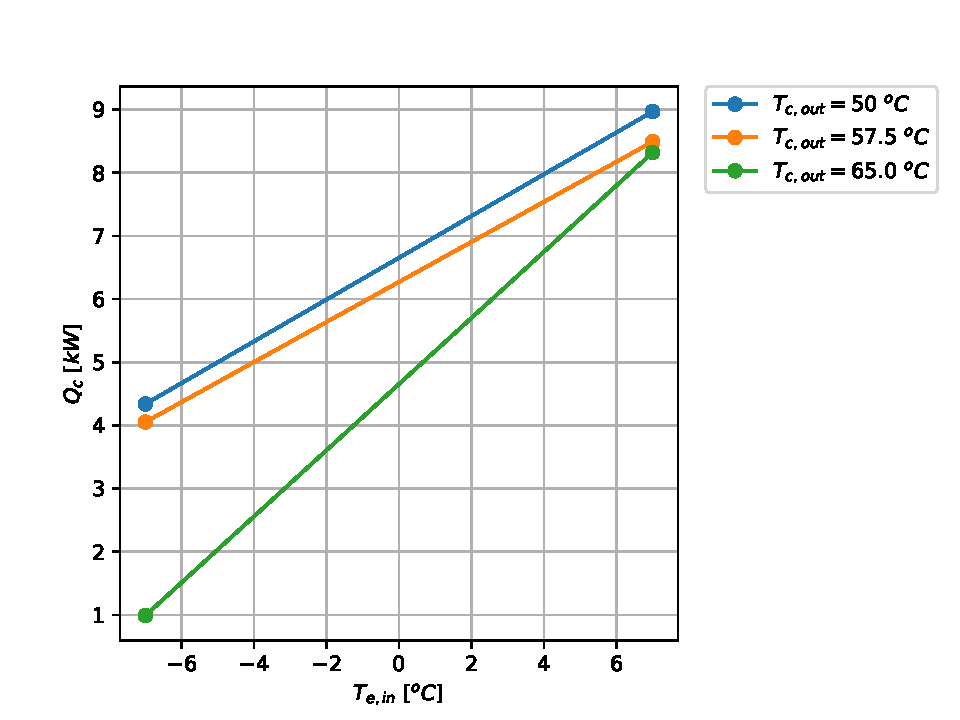
\includegraphics[width=1\textwidth]{C:/Daten/OngoingProject/TRNSYS-Polysun/HeatPumpFit/AirToWater/LEXETA/AWHP-LEXETA/AWHP-LEXETA-Qc.pdf}
\caption{$Q_c$ Results for the heat pump at the selected points}
\label{QcFig}
\end{center}
\end{figure}
\end{document}
